
\textbf{Ejemplo 2}\\
Un inversionista en Colombia adquiere un documento que vale 300 USD, gana un
interés del 6\% nominal anual año vencido en dólares a un plazo de un año. El
tipo de cambio actual es  1 USD =  1.500 COP y se estima una devaluación del peso con respecto al dólar durante ese año del 20\% nominal anual año vencido. Calcular la rentabilidad que se podía obtener. ¿Cuál es la utilidad neta, una vez descontada la retención en la fuente del 7\%?\\ \\
\newpage %USAR SOLO SI EL SOLUCIÓN QUEDA SOLO Y ES NECESARIO BAJARLO A LA SIGUIENTE PAGINA
\textbf{Solución.}\\
%La tabla ira centrada
\begin{center}
 \renewcommand{\arraystretch}{1.5}% Margenes de las celdas
 %Creación de la cuadricula de 3 columnas
 \begin{longtable}[H]{|c|c|c|}
  %Creamos una linea horizontal
  \hline
  %Definimos el color de la primera fila
  \rowcolor[HTML]{FFB183}
  %%%%% INICIO DECLARACIÓN DE VARIABLES %%%%%%%
  %%%%%%%%%% INICIO TITULO
  %Lo que se hace aquí es mezclar las 3 columnas en una sola
\multicolumn{3}{|c|}{\cellcolor[HTML]{FFB183}\textbf{1. Asignación de Periodo Focal}}                                        \\ \hline
  %%%%%%%%%% FIN TITULO
  %%%%%%%%%% INICIO DE MATEMÁTICAS
  %Cada & hace referencia al paso de la siguiente columna
  \multicolumn{3}{|c|}{\textit{$pf : 1 pav$}}                                                            \\ \hline
  \multicolumn{3}{|c|}{\cellcolor[HTML]{FFB183}\textbf{2. Declaración de variables}}                                        \\ \hline
  %%%%%%%%%% FIN TITULO
  %%%%%%%%%% INICIO SUBTITULO
  \multicolumn{1}{|c|}{\cellcolor[HTML]{FFB183}\textbf{Valores monetarios}}    & 
  \multicolumn{1}{|c|}{\cellcolor[HTML]{FFB183}\textbf{Valores no monetarios}} &
  \multicolumn{1}{|c|}{\cellcolor[HTML]{FFB183}\textbf{Incógnitas}}  \\ \hline
  %%%%%%%%%% FIN SUBTITULO
  %%%%%%%%%% INICIO DE MATEMÁTICAS
  %Cada & hace referencia al paso de la siguiente columna
 
 	$\text{dólar: } 1 \text{ USD} = 1.500 \text{ COP}$ &$j = 6\% \textit{ naav en USD}$  & $i = ?\%$ \\
 	&$i = \frac{6 \textit{ naav}}{1 \textit{ pav}} = 6\% \textit{ pav en USD}$  & \\
 	& $j_{dev}=20\% \textit{ naav}$ &\\ & $n = 1  \textit{ pav}$ & \\ \hline

 

  %%%%%%%%%% FIN DE MATEMÁTICAS
  %%%%% FIN DECLARACIÓN DE VARIABLES


  %%%%% INICIO FLUJO DE CAJA
  \rowcolor[HTML]{FFB183}
  \multicolumn{3}{|c|}{\cellcolor[HTML]{FFB183}\textbf{3. Diagrama de flujo de caja}}                                       \\ \hline
  %Mezclamos 3 columnas y pondremos el dibujo
  %%%%%%%%%%%%% INSERCIÓN DE LA IMAGEN
  %Deberán descargar las imágenes respectivas del drive y pegarlas en la carpeta
  %n_capitulo/img/ejemplos/1/capitulo1ejemplo1.pdf  (el /1/ es el numero del ejemplo)
  \multicolumn{3}{|c|}{ 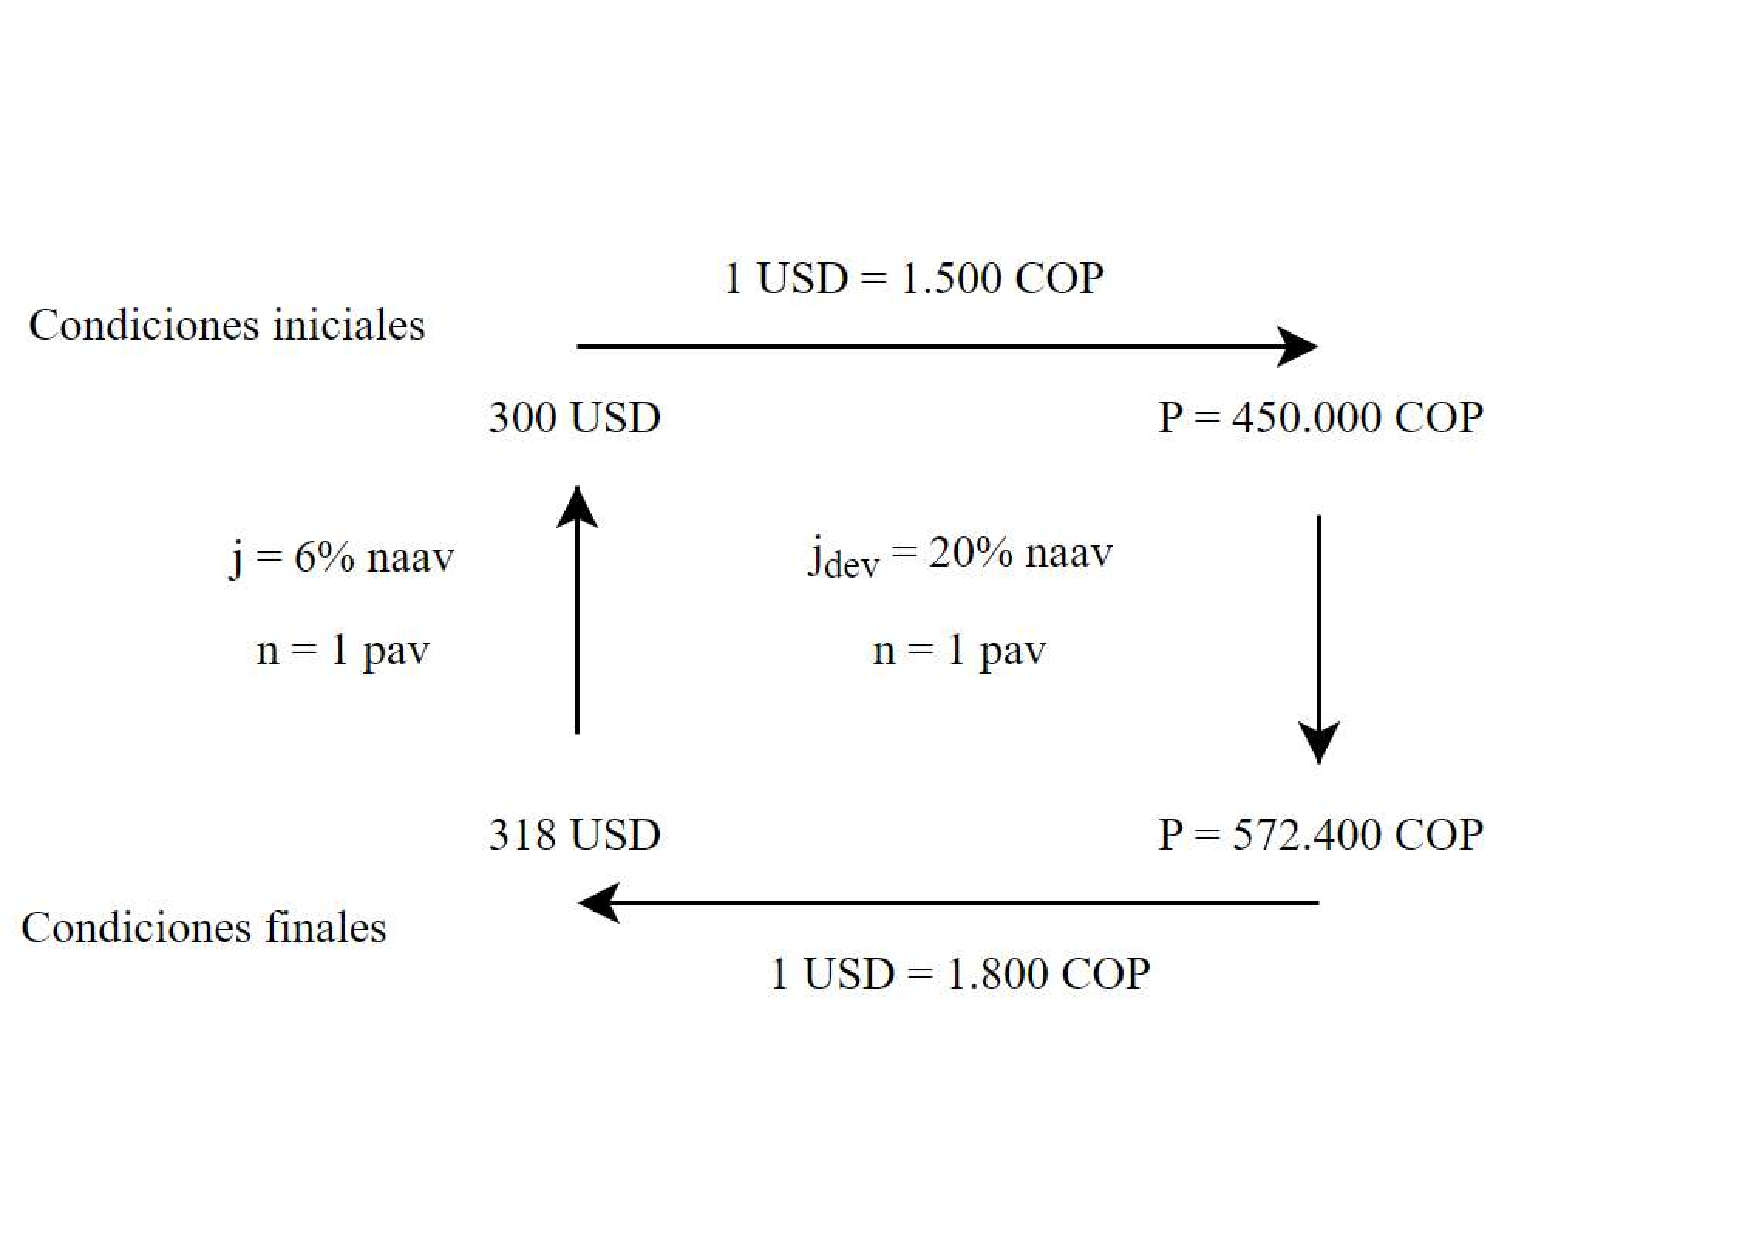
\includegraphics[trim=-5 -5 -5 -5 , scale=0.55, width=16.4 cm, height = 10.5 cm]{3_Capitulo/img/ejemplos/2/capitulo3ejercicio2.pdf} }                         \\ \hline
  %%%%%%%%%%%%% FIN INSERCIÓN DE IMAGEN
  %%%%%FIN FLUJO DE CAJA



  %%%%% INICIO DECLARACIÓN FORMULAS
  %%%%%%%%%%% INICIO TITULO
  \rowcolor[HTML]{FFB183}
  \multicolumn{3}{|c|}{\cellcolor[HTML]{FFB183}\textbf{4. Declaración de Fórmulas}}                                         \\ \hline
  %%%%%%%%%%% FIN TITULO
  %%%%%%%%%%% INICIO MATEMÁTICAS
  \multicolumn{3}{|c|}{$F = P (1 + i)^n \textit{ Valor futuro}$}                                                            \\ 
  \multicolumn{3}{|c|}{$RF= 0,07(F-P) \textit{Retención de la fuente }$}
    \\
  %%%%%%%%%% FIN MATEMÁTICAS
  %%%%%% INICIO DESARROLLO MATEMÁTICO
  \rowcolor[HTML]{FFB183}
  %%%%%%%%%%INICIO TITULO
 \multicolumn{3}{|c|}{\cellcolor[HTML]{FFB183}\textbf{5. Desarrollo Matemático}}                                        \\ \hline
  %%%%%%%%%% FIN TITULO
  %%%%%%%%%% INICIO MATEMÁTICAS
  \multicolumn{3}{|p{\textwidth}|}{
  	\begin{center}
  	$300 \ USD$ en pesos $\equiv (300\ USD)1{.}500 \left(\frac{COP}{USD}\right) = 450{.}000 \ COP$\newline
  
  		$F = 300 \ USD(1 + 0,06)^1 = 318 \ US$ \vspace{3mm} \newline
  		
  		$F =  1{.}500 \ COP (1 + 0,02)^1=  1{.}800 \ COP$\newline
  		
  		$  (318 \ USD)(\frac{ 1{.}800 \ COP}{1 \ USD})= 572{.}400 \ COP$\newline
  		
  		$ \frac{(318 \ USD) (1{.}800 \ COP)}{ 1 \ USD} =  572{.}400 \ COP$\newline
  		
  	\end{center}
  	$\text{Se calcula la retencion de la fuente:}$\newline
  	\begin{center}
  		$R =  572{.}400 \ COP - 450{.}000 \ COP =  122{.}400 \ COP$\newline
  	\end{center}
  	$\text{Se calcula la rentabilidad neta:}$\newline
  	\begin{center}
  		$R_{neta} =  572{.}400 \ COP - 8{.}568 \ COP =  563{.}832 \ COP$\newline
  	\end{center}
}
                                                                                                                    \\ \hline
\multicolumn{3}{|c|}{\cellcolor[HTML]{FFB183}\textbf{6. Respuesta}}                                         \\ \hline
  %%%%%%%%%%% FIN TITULO
  %%%%%%%%%%% INICIO MATEMÁTICAS
\multicolumn{3}{|p{\textwidth}|}{El valor de la utilidad sin descontar la retención en la fuente era de 122.400 COP. Al descontar la retención en la fuente esa utilidad neta es de
563.832 COP}  \\ \hline
  %%%%%%%%%% FIN MATEMÁTICAS

  %%%%%%%%%% FIN MATEMÁTICAS
  %%%%%% FIN DESARROLLO MATEMÁTICO
  %%%%%% INICIO RESPUESTA



  %%%%%%%%%% FIN MATEMÁTICAS
  %%%%%% FIN RESPUESTA
 \end{longtable}
 %Se crean dos lineas en blanco para que no quede el siguiente texto tan pegado
 %\newline \newline %USARLO SI CREES QUE ES NECESARIO
\end{center}